\documentclass{beamer}
\usepackage[utf8x]{inputenc}
\usepackage[T2A]{fontenc}
\usepackage[english,russian]{babel}

\usetheme{mybeamer}


\title{Влияние точности входных параметров моделей ядерных реакций на предсказанные выходы $r$-процесса}
\subtitle{Магистерская диссертация}
\author{Негребецкий В.В.}
\institute{МГУ им. М.В. Ломоносова, физический факультет,\\
кафедра общей ядерной физики\\
\vspace{1em}
\textnormal{Научный руководитель: к.ф.-м.н. Стопани К.А.}
}
\date{}

\begin{document}
  \frame[noframenumbering] {
    \titlepage
  }
  
  \frame{
    \frametitle{Распространенности ядер в Солнечной системе}
    \small
    Проблема нуклеосинтеза тяжелых изотопов:
    \begin{itemize}
      \item Легкие изотопы образуются в реакциях звездного горения.
      \item Синтез ядер тяжелее железа энергетически невыгоден.
      \item Таких ядер действительно довольно мало. 
    \end{itemize}
    \center
    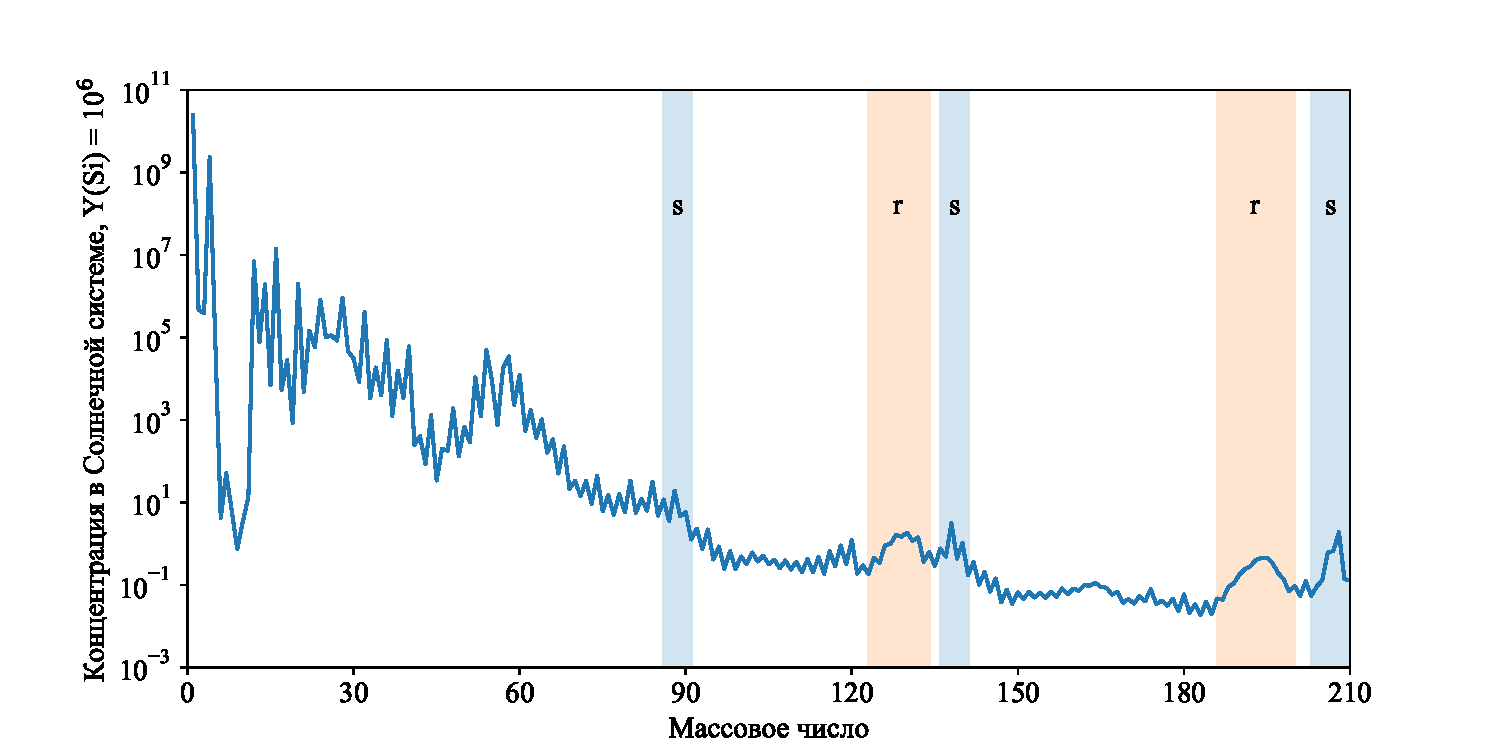
\includegraphics[width=\textwidth]{../pics/lodders.pdf}
    \scriptsize
    По данным \textit{Lodders 2003}.
  }

  \frame{
    \frametitle{Механизм нейтронного захвата}
    \small
    Синтез тяжелых ядер в основном обеспечивают $s$- и $r$-процесс.
    \begin{centering}
    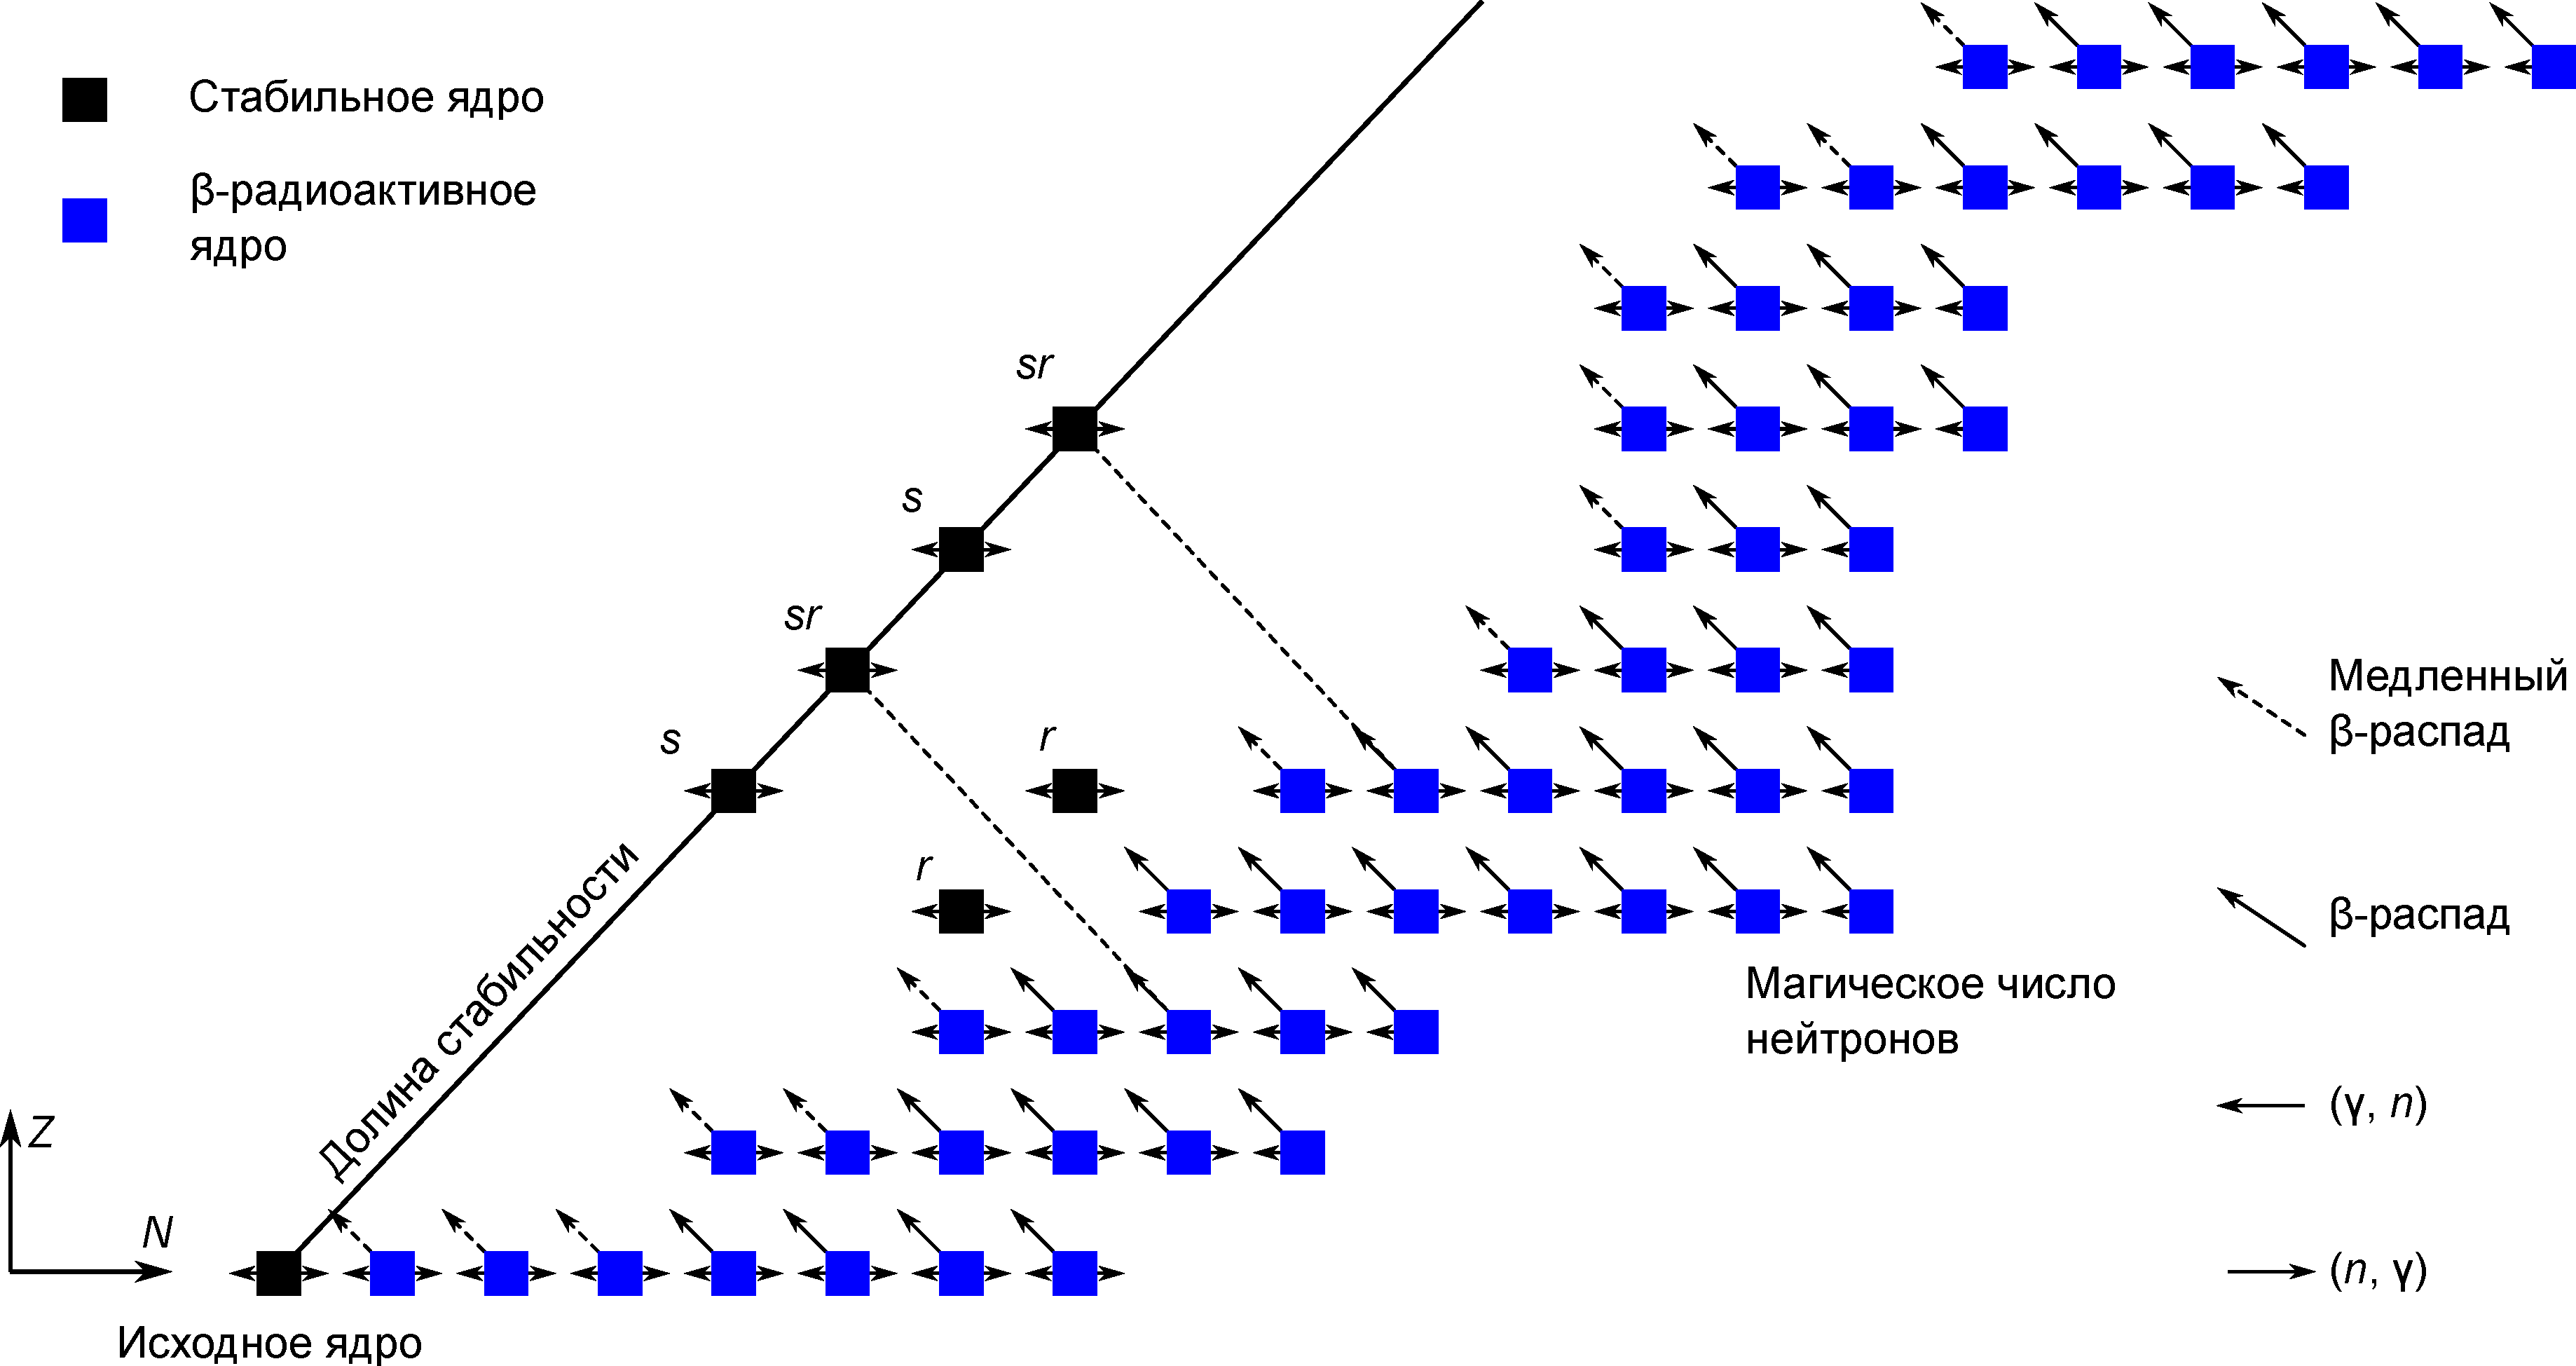
\includegraphics[width=0.9\textwidth]{../pics/tracks.pdf}
    \end{centering}
    
    \begin{block}{\bf \small Особенности $r$-процесса}
      \small
      Экстремальные астрофизические условия и участие \textbf{сверхнейтроноизбыточных} ядер.
    \end{block}
  }

  \frame{
    \frametitle{Моделирование нуклеосинтеза}
    \small
    Система уравнений нуклеосинтеза: 
    \begin{equation*}
    \displaystyle 
    \frac{d y_i}{d t} = \sum_{k \in K_i} \pm {\color{blue}\lambda_k} \prod_{l \in L_k} y_l
    \end{equation*}
    
    Особенности задачи:
    \begin{itemize}
      \item Огромная размерность ($\sim 7800$ изотопов и $\sim 10^5$ реакций)
      \item Сверхжесткость системы уравнений 
      \item Неопределенность астрофизических параметров
      \item Недостаток данных о задействованных экзотических ядрах, \\
        \textbf{их характеристики приходится получать из моделей}
    \end{itemize}
  
    \begin{block}{\bf \small Цель работы}
      \small
      Выяснить, каково влияние неопределенностей ядерных данных, полученных из
      теоретических моделей, на результаты моделирования $r$-процесса.
    \end{block}
  }

  \frame{
    \frametitle{Астрофизические скорости реакций}
    О скоростях:
    \begin{itemize}
      \item Что это такое
      \item Как влияют
      \item Как вычислять (формула)
    \end{itemize}
  }

  \frame{
    \frametitle{Модели масс экзотических ядер}
    Об использованных массовых моделях:
    \begin{itemize}
      \item Сказать, что массы -- важные параметры расчета сечений
      \item Перечислить и кратко описать
      \item Чуть подробнее про LMR (график фитов)
      \item Сравнение точностей (график)
    \end{itemize}
  }

  \frame{
    \frametitle{Расчет сечений и скоростей $(n,\gamma)$}
    Показать промежуточные результаты:
    \begin{itemize}
      \item О статистической модели и о TALYS
      \item 2-3 графика сечений 
      \item 2-3 графика скоростей
      \item О создании библиотек реакций на базе REACLIB
      \item О ratelib
    \end{itemize}
  }

  \frame{
    \frametitle{Скорости $\beta$-распадов}
    Как я фитировал скорости распадов:
    \begin{itemize}
      \item Почему их вообще надо фитировать (график рис. 8)
      \item Почему я считаю, что нашей точности вполне достаточно
      \item Модельные функции
      \item Результаты (2 графика)
    \end{itemize}
  }
  
  \frame{
    \frametitle{Астрофизические параметры модели}
    \begin{itemize}
      \item Чаще всего рассматривают сценарий NSM
      \item Начальные условия
      \item Вычисление начальной композиции и плотности
      \item Как меняется плотность в симуляции
      \item Как меняются остальные параметры
    \end{itemize}
  }
  
  \frame{
    \frametitle{Эволюция выходов $r$-изотопов}
    \begin{itemize}
      \item Анимация
      \item Что означает тонкая линия и ее исчезновение
      \item HFB запаздывает!
    \end{itemize}
  }

  \frame{
    \frametitle{Итоговое массовое распределение}
    \begin{itemize}
      \item График распределения
      \item Про неопределенности
      \item Про положение пиков
    \end{itemize}
  }

  \usebeamertemplate{endpage}

  \frame{
    \frametitle{Appendix\\Нейтронный захват за границей существования}
    Просто рис. 7 из диплома и пояснение: мы учитываем реакции даже при $B_n < 0$. C одной стороны, так можно по инерции выходить за пределы границ существования ядер, но, с другой, ничего страшного при этом не происходит, так как скорости там резко падают.
  }

  \frame{
    \frametitle{Appendix\\Слабые распады в библиотеке REACLIB}
    \begin{itemize}
      \item График рис. 9: с какого-то $A$ доминируют распады с вылетом нейтронов.
      \item Мы считаем, что их можно добавлять в скорости $\beta$-распадов при фитировании, потому что недостаток нейтронов быстро компенсируется захватами.
    \end{itemize}
  }
  
  \frame{
    \frametitle{Appendix\\Влияние массовой модели на температуру}
    \begin{itemize}
      \item График рис. 15 
      \item Вроде бы, разница очень маленькая, но
      \item Источник тепла -- $\beta$-распады, а у нас три симуляции различаются в этом плане очень слабо, по границе отделения нейтронов
    \end{itemize}
  }
\end{document}
